\documentclass[10pt]{beamer}

% Pacotes Extras
\usepackage{rotating}
\usepackage{dsfont}
\usepackage{comment}
\usepackage{xcolor}
\usepackage{xcolor-material}
\usepackage{xcolor-solarized}
\usepackage[cachedir=.mintedcache]{minted}
\usemintedstyle{material}
\usepackage{multicol}
\usepackage{listings}
\usepackage{ulem}
\usepackage{cancel}
\usepackage{lipsum} 
\usepackage{graphicx}
\usepackage{pstricks}
\usepackage{pst-plot}
\usepackage{pst-3dplot}
\usepackage{booktabs}
\usepackage{wrapfig}
\usepackage{chngcntr}
\counterwithin*{footnote}{section}
\usepackage{metalogo}
\usepackage{enumitem}
%\usepackage{caption}
%\usepackage{subcaption}
\usepackage{subfig}
\usepackage[most]{tcolorbox}
\tcbuselibrary{breakable}
\tcbuselibrary{minted}
\usetikzlibrary{decorations.pathmorphing} 
\tcbuselibrary{skins}
\usepackage{setspace}
\PassOptionsToPackage{hyphens}{url}\usepackage{hyperref}
\usepackage{xspace}
\usepackage{lscape}
\usepackage{pdfpages}

% Macros extras
\definecolor{preto}{HTML}{515151}

% Caixas das Dicas (pacote tcolorbox)
% Material Colors
%\newtcolorbox{marker}[1][]{enhanced,
%  before skip=10mm,after skip=10mm,
%  boxrule=0.4pt,left=5mm,right=2mm,top=1mm,bottom=1mm,
%  colback=MaterialAmberA100,
%  colupper=preto,
%  colframe=MaterialGrey900,
%  sharp corners,rounded corners=southeast,arc is angular,arc=3mm,
%  underlay={%
%    \path[fill=tcbcol@back!80!black] ([yshift=3mm]interior.south east)--++(-0.4,-0.1)--++(0.1,-0.2);
%    \path[draw=tcbcol@frame,shorten <=-0.05mm,shorten >=-0.05mm] ([yshift=3mm]interior.south east)--++(-0.4,-0.1)--++(0.1,-0.2);
%    \path[fill=MaterialYellow100!50!black,draw=none] (interior.south west) rectangle node[white]{\Huge\bfseries !} ([xshift=4mm]interior.north west);
%    },
%  drop fuzzy shadow,#1}
\newtcolorbox{marker}[1][]{enhanced,
  before skip=10mm,after skip=10mm,
  boxrule=1.4pt,left=6mm,right=3mm,top=2mm,bottom=2mm,
  colback=MaterialAmberA100!75,
  colupper=black,
  colframe=preto,
  underlay={%
    \path[fill=none] (frame.south west) rectangle node[preto]{\huge\bfseries !} ([xshift=7mm]frame.north west);
    }}
  
% Caixas dos Exemplos (pacote tcolorbox)
% Material Colors
\tcbset{
    texexp/.style={
        colframe=MaterialBlue900,
        colback=white,
        coltitle=white,
        fonttitle=\small\sffamily\bfseries,
        fontupper=\small, 
        fontlower=\small},
        example/.style 2 args={texexp,
        title={Exemplo \thetcbcounter: #1},label={#2}},
    }
    \newtcblisting{texexp}[1]{texexp,#1}
    \newtcblisting[auto counter,number within=section]{texexptitled}[3][]{%
        example={#2}{#3},#1}
    \newtcolorbox[use counter from=texexptitled]{texexptitledspec}[3][]{%
        example={#2}{#3},#1}

%\newtcolorbox[auto counter,number within=section,list inside=exam]{texercise}[4][]{%
%    texercisestyle,
%    listing file={respostas/texercise\thetcbcounter.tex},
%    label={exe:#2},
%    record={\string\processsol{respostas/texercise\thetcbcounter.tex}{#2}},
%    title={Exercício \thetcbcounter\hfill\mdseries Resposta na página \pageref{sol:#2}},
%    list text={\vspace{-1em}\hspace{1mm} #3 (Resposta na página \pageref{sol:#2}}), #1)}

% Caixas dos Exercícios e Soluções (pacote tcolorbox)  
% Material Colors
\NewTColorBox[auto counter,number within=chapter]{exercise}{m+O{}}{%
    enhanced,
    colframe=MaterialGreen900,
    colback=white,
    coltitle=white,
    fonttitle=\bfseries,
    underlay={\begin{tcbclipinterior}
        \shade[inner MaterialGreen900,outer color=white]
            (interior.north west) circle (2cm);
        \draw[help lines,step=5mm,MaterialGreen900,shift={(interior.north west)}]
            (interior.south west) grid (interior.north east);
        \end{tcbclipinterior}},
    title={Exercício~ \thetcbcounter:},
    label={exercise:#1},
    attach title to upper=\quad,
    after upper={\par\hfill\textcolor{white}%
        {\itshape Resposta na página~\pageref{solution:#1}}},
    lowerbox=ignored,
    savelowerto=docs/respostas/exercise-\thetcbcounter.tex,
    record={\string\solution{#1}{docs/respostas/exercise-\thetcbcounter.tex}},
    #2
}

% Esta é a lista de exercícios
\newtcolorbox[auto counter,number within=section,list inside=exam]{texercise}[4][]{%
    texercisestyle,
    listing file={docs/respostas/texercise\thetcbcounter.tex},
    label={exe:#2},
    record={\string\processsol{docs/respostas/texercise\thetcbcounter.tex}{#2}},
    title={Exercício \thetcbcounter\hfill\mdseries Resposta na página \pageref{sol:#2}},
    list text={\vspace{-1em}\hspace{1mm} #3 - resposta na página \pageref{sol:#2}}, #1)}
    
\tcbset{texercisestyle/.style={arc=0.5mm, colframe=MaterialGreen900,
    colback=white, coltitle=white,
    fonttitle=\small\sffamily\bfseries, fontupper=\small, fontlower=\small,
    listing options={style=tcblatex,texcsstyle=*\color{MaterialRed900}},
}}

% \usepackage{hyperref} % for phantomlabel
\newtcbinputlisting{\processsol}[2]{%
    texercisestyle,
    listing only,
    listing file={#1},
    phantomlabel={sol:#2},%
    title={Resposta do Exercício \ref{exe:#2} na página \pageref{exe:#2}},
}

% Caixa dos Comandos (pacote tcolorbox)
% Material Colors
\newtcblisting{commandshell}{colback=MaterialBlueGrey900,colupper=MaterialBlueGrey50,colframe=MaterialBlueGrey900!75!MaterialBlueGrey900,listing only,listing options={style=tcblatex,language=sh},
    every listing line={\textcolor{MaterialRed500}{\small\ttfamily\bfseries \$ }}}

%\newtcblisting{meucomando}{listing engine=minted,
%	minted style=colorful,
%	minted language=bash,
%	minted options={fontsize=\small,breaklines,autogobble,linenos,numbersep=3mm},
%	colback=MaterialAmber50,colframe=MaterialBlueGrey900,listing only,
%	left=5mm,enhanced,
%	overlay={\begin{tcbclipinterior}\fill[MaterialAmber600] (frame.south west)
%			rectangle ([xshift=5mm]frame.north west);\end{tcbclipinterior}}}

\newtcblisting{meucomando}{listing engine=minted,
	minted style=colorful,
	minted language=bash,
	minted options={fontsize=\small,breaklines,autogobble,linenos,numbersep=3mm},
	colback=blue!5!white,colupper=black,colframe=preto,listing only,
	left=5mm,enhanced,
	overlay={\begin{tcbclipinterior}\fill[red!20!blue!20!white] (frame.south west)
			rectangle ([xshift=5mm]frame.north west);\end{tcbclipinterior}}}

% Sentenças individuais Loren Lipsum (pacote lipsum)
% REF: https://tex.stackexchange.com/questions/254901/one-sentence-of-dummy-text
% store a big set of sentences
\unpacklipsum[1-100] % it was \UnpackLipsum before version 2.0
\ExplSyntaxOn
% unpack \lipsumexp
\seq_new:N \g_lipsum_sentences_seq
\cs_generate_variant:Nn \seq_set_split:Nnn { NnV }
\seq_gset_split:NnV \g_lipsum_sentences_seq {.~} \lipsumexp

\NewDocumentCommand{\lipsumsentence}{>{\SplitArgument{1}{-}}O{1-7}}
 {
  \lipsumsentenceaux #1
 }
\NewDocumentCommand{\lipsumsentenceaux}{mm}
 {
  \IfNoValueTF { #2 }
   {
    \seq_item:Nn \g_lipsum_sentences_seq { #1 }.~
   }
   {
    \int_step_inline:nnnn { #1 } { 1 } { #2 }
     {
      \seq_item:Nn \g_lipsum_sentences_seq { ##1 }.~
     }
   }
 }
\ExplSyntaxOff


\usepackage[alf]{abntex2cite}
\usepackage{bibentry}

\usetheme{metropolis}

\usefonttheme[onlymath]{serif}
\usefonttheme{professionalfonts}
\usepackage{mathspec} 
\metroset{titleformat=allsmallcaps} % smallcaps

\setbeamercolor{alerted text}{fg=InpeLaranja}
\setbeamercolor{frametitle}{bg=InpeAzul}
\setbeamercolor{normal text}{fg=black}
\setbeamercolor{progress bar}{bg=InpeLaranja,fg=InpeAzul}
\setbeamercolor{title separator}{bg=InpeLaranja,fg=InpeLaranja}
\setbeamercolor{background canvas}{bg=white}

\setbeamertemplate{caption}[numbered]

\AtBeginSubsection[
  {\frame<beamer>{\frametitle{Sumário}   
    \tableofcontents[currentsection,currentsubsection]}}%
]%
{
  \frame<beamer>{ 
    \frametitle{Sumário}
    \begin{multicols}{2}
    \tableofcontents[currentsection,currentsubsection]
    \end{multicols}
    }
}

\title{Introdução ao \LaTeX}
\subtitle{Parte IV}
\date{05 de Março de 2020}
\author{Carlos Frederico Bastarz (CPTEC/INPE)}
\institute{Instituto Nacional de Pesquisas Espaciais (INPE)}
\titlegraphic{\hfill
\includegraphics[height=1.5cm]{figs/layout/inpe_logo.png}}

\makeatletter
\patchcmd{\beamer@sectionintoc}{\vskip1.5em}{\vskip0.75em}{}{}
\makeatother

\begin{document}

\maketitle

\begin{frame}[c]{Sumário}
    \vspace{2em}
    \begin{multicols}{2}
        \begin{minipage}{0.49\textwidth}
           \vspace{8mm}
           \setbeamertemplate{section in toc}[sections numbered]
           \tableofcontents
        \end{minipage}
        \begin{minipage}{0.49\textwidth}
            
\includegraphics[width=\textwidth]{./figs/ctan_lion_350x350.pdf}
        \end{minipage}
    \end{multicols}
\end{frame}

\section{Parte IV - Pacote \textit{Beamer}}

\begin{frame}{Pacote \textit{Beamer}}
	\begin{block}{É possível fazer apresentações com o \LaTeX{}?}
		\begin{itemize}
			\pause
			\item Sim, há algumas classes que são orientadas para isso;
			\pause
			\item Exemplos: {\tt beamer}, {\tt tcolorbox}, {\tt powerdot};
			\pause
			\item A ideia é a mesma, mas a lógica é um pouco diferente;
			\pause
			\item \textit{Beamer} é o pacote mais utilizado.
		\end{itemize}
	\end{block}
\end{frame}

\begin{frame}{Pacote \textit{Beamer}}
	\begin{block}{Quando é conveniente fazer apresentações com o \textit{Beamer?}}
		\begin{itemize}
			\pause
			\item Embora seja uma classe do \LaTeX{}, como sempre, é necessário tempo;
			\pause
			\item Os mesmos pacotes utilizados com as classes mais comuns do \LaTeX{}, também podem ser utilizados com a classe do \textit{Beamer};
			\pause
			\item Pense no \textit{Beamer} como o \LaTeX{} no modo paisagem:
			\begin{itemize}
			    \pause
			    \item Suas tabelas longas e imagens grandes podem não caber no documento \textit{Beamer};
			    \pause
			    \item Adaptações podem ser necessárias.
			\end{itemize}
		\end{itemize}
	\end{block}
\end{frame}

\begingroup
\setbeamercolor{background canvas}{bg=InpeLaranja}
\begin{frame}[plain,fragile]{}
\begin{texexptitled}[center, enhanced jigsaw, width=0.99\paperwidth, height=0.99\paperheight, middle=2mm, listing side comment, righthand width=5cm, compilable listing, run latex, run dvips, run ps2pdf, pdf comment, comment style={raster columns=1},freeze pdf]{Um documento \LaTeX{} mínimo}{exe_doc1}
\documentclass[10pt]{article}
% Este é o preâmbulo
\usepackage[utf8]{inputenc}
\usepackage{lipsum}

\title{Título}
\author{Nome}
\date{\today}

% A partir daqui inicia-se o documento
\begin{document}
\maketitle

\section{Seção}

\lipsum[1-2]
\end{document}
\end{texexptitled}
\end{frame}

\begin{frame}[plain,fragile]{}
\begin{texexptitled}[center, enhanced jigsaw, width=0.99\paperwidth, height=0.99\paperheight, middle=2mm, listing side comment, righthand width=5cm, compilable listing, run latex, run dvips, run ps2pdf, pdf comment, comment style={raster columns=1},freeze pdf]{Um documento \textit{Beamer} mínimo}{exe_doc2}
\documentclass[10pt]{beamer}
% Este é o preâmbulo
\usepackage[utf8]{inputenc}
\usepackage{lipsum}

\title{Título}
\author{Nome}
\date{\today}

% A partir daqui inicia-se o documento
\begin{document}
\maketitle

\section{Seção}

\lipsum[1-2]
\end{document}
\end{texexptitled}
\end{frame}
\endgroup

\begin{frame}[fragile]{Pacote \textit{Beamer}}
    \begin{block}{Diferença principal entre os documentos:}
        \begin{itemize}
            \pause
            \item Classe do documento: {\tt article} X {\tt beamer}?
            \pause
            \item Não é apenas isso!
        \end{itemize}
    \end{block}
    \pause
    \begin{block}{O Exemplo \ref{exe_doc2} não está completo/correto!}
        \begin{itemize}
            \pause
            \item No \textit{Beamer}, os blocos de texto são delimitados por um ambiente especial, o {\tt frame};
            \pause
            \item \textit{Frames} são, portanto, os \textit{slides}\footnote{No sentido \textit{PowerPoint} das coisas.} do \textit{Beamer}.
        \end{itemize}
    \end{block}
\end{frame}

\subsection{Preâmbulo}

\begin{tcboutputlisting}
    ...
    \usepackage[utf8]{inputenc}
    \usepackage[brazilian]{babel}
    \usepackage{...}
    ...
    % Pacotes Extras
\usepackage{rotating}
\usepackage{dsfont}
\usepackage{comment}
\usepackage{xcolor}
\usepackage{xcolor-material}
\usepackage{xcolor-solarized}
\usepackage[cachedir=.mintedcache]{minted}
\usemintedstyle{material}
\usepackage{multicol}
\usepackage{listings}
\usepackage{ulem}
\usepackage{cancel}
\usepackage{lipsum} 
\usepackage{graphicx}
\usepackage{pstricks}
\usepackage{pst-plot}
\usepackage{pst-3dplot}
\usepackage{booktabs}
\usepackage{wrapfig}
\usepackage{chngcntr}
\counterwithin*{footnote}{section}
\usepackage{metalogo}
\usepackage{enumitem}
%\usepackage{caption}
%\usepackage{subcaption}
\usepackage{subfig}
\usepackage[most]{tcolorbox}
\tcbuselibrary{breakable}
\tcbuselibrary{minted}
\usetikzlibrary{decorations.pathmorphing} 
\tcbuselibrary{skins}
\usepackage{setspace}
\PassOptionsToPackage{hyphens}{url}\usepackage{hyperref}
\usepackage{xspace}
\usepackage{lscape}
\usepackage{pdfpages}

    % Macros extras
\definecolor{preto}{HTML}{515151}

% Caixas das Dicas (pacote tcolorbox)
% Material Colors
%\newtcolorbox{marker}[1][]{enhanced,
%  before skip=10mm,after skip=10mm,
%  boxrule=0.4pt,left=5mm,right=2mm,top=1mm,bottom=1mm,
%  colback=MaterialAmberA100,
%  colupper=preto,
%  colframe=MaterialGrey900,
%  sharp corners,rounded corners=southeast,arc is angular,arc=3mm,
%  underlay={%
%    \path[fill=tcbcol@back!80!black] ([yshift=3mm]interior.south east)--++(-0.4,-0.1)--++(0.1,-0.2);
%    \path[draw=tcbcol@frame,shorten <=-0.05mm,shorten >=-0.05mm] ([yshift=3mm]interior.south east)--++(-0.4,-0.1)--++(0.1,-0.2);
%    \path[fill=MaterialYellow100!50!black,draw=none] (interior.south west) rectangle node[white]{\Huge\bfseries !} ([xshift=4mm]interior.north west);
%    },
%  drop fuzzy shadow,#1}
\newtcolorbox{marker}[1][]{enhanced,
  before skip=10mm,after skip=10mm,
  boxrule=1.4pt,left=6mm,right=3mm,top=2mm,bottom=2mm,
  colback=MaterialAmberA100!75,
  colupper=black,
  colframe=preto,
  underlay={%
    \path[fill=none] (frame.south west) rectangle node[preto]{\huge\bfseries !} ([xshift=7mm]frame.north west);
    }}
  
% Caixas dos Exemplos (pacote tcolorbox)
% Material Colors
\tcbset{
    texexp/.style={
        colframe=MaterialBlue900,
        colback=white,
        coltitle=white,
        fonttitle=\small\sffamily\bfseries,
        fontupper=\small, 
        fontlower=\small},
        example/.style 2 args={texexp,
        title={Exemplo \thetcbcounter: #1},label={#2}},
    }
    \newtcblisting{texexp}[1]{texexp,#1}
    \newtcblisting[auto counter,number within=section]{texexptitled}[3][]{%
        example={#2}{#3},#1}
    \newtcolorbox[use counter from=texexptitled]{texexptitledspec}[3][]{%
        example={#2}{#3},#1}

%\newtcolorbox[auto counter,number within=section,list inside=exam]{texercise}[4][]{%
%    texercisestyle,
%    listing file={respostas/texercise\thetcbcounter.tex},
%    label={exe:#2},
%    record={\string\processsol{respostas/texercise\thetcbcounter.tex}{#2}},
%    title={Exercício \thetcbcounter\hfill\mdseries Resposta na página \pageref{sol:#2}},
%    list text={\vspace{-1em}\hspace{1mm} #3 (Resposta na página \pageref{sol:#2}}), #1)}

% Caixas dos Exercícios e Soluções (pacote tcolorbox)  
% Material Colors
\NewTColorBox[auto counter,number within=chapter]{exercise}{m+O{}}{%
    enhanced,
    colframe=MaterialGreen900,
    colback=white,
    coltitle=white,
    fonttitle=\bfseries,
    underlay={\begin{tcbclipinterior}
        \shade[inner MaterialGreen900,outer color=white]
            (interior.north west) circle (2cm);
        \draw[help lines,step=5mm,MaterialGreen900,shift={(interior.north west)}]
            (interior.south west) grid (interior.north east);
        \end{tcbclipinterior}},
    title={Exercício~ \thetcbcounter:},
    label={exercise:#1},
    attach title to upper=\quad,
    after upper={\par\hfill\textcolor{white}%
        {\itshape Resposta na página~\pageref{solution:#1}}},
    lowerbox=ignored,
    savelowerto=docs/respostas/exercise-\thetcbcounter.tex,
    record={\string\solution{#1}{docs/respostas/exercise-\thetcbcounter.tex}},
    #2
}

% Esta é a lista de exercícios
\newtcolorbox[auto counter,number within=section,list inside=exam]{texercise}[4][]{%
    texercisestyle,
    listing file={docs/respostas/texercise\thetcbcounter.tex},
    label={exe:#2},
    record={\string\processsol{docs/respostas/texercise\thetcbcounter.tex}{#2}},
    title={Exercício \thetcbcounter\hfill\mdseries Resposta na página \pageref{sol:#2}},
    list text={\vspace{-1em}\hspace{1mm} #3 - resposta na página \pageref{sol:#2}}, #1)}
    
\tcbset{texercisestyle/.style={arc=0.5mm, colframe=MaterialGreen900,
    colback=white, coltitle=white,
    fonttitle=\small\sffamily\bfseries, fontupper=\small, fontlower=\small,
    listing options={style=tcblatex,texcsstyle=*\color{MaterialRed900}},
}}

% \usepackage{hyperref} % for phantomlabel
\newtcbinputlisting{\processsol}[2]{%
    texercisestyle,
    listing only,
    listing file={#1},
    phantomlabel={sol:#2},%
    title={Resposta do Exercício \ref{exe:#2} na página \pageref{exe:#2}},
}

% Caixa dos Comandos (pacote tcolorbox)
% Material Colors
\newtcblisting{commandshell}{colback=MaterialBlueGrey900,colupper=MaterialBlueGrey50,colframe=MaterialBlueGrey900!75!MaterialBlueGrey900,listing only,listing options={style=tcblatex,language=sh},
    every listing line={\textcolor{MaterialRed500}{\small\ttfamily\bfseries \$ }}}

%\newtcblisting{meucomando}{listing engine=minted,
%	minted style=colorful,
%	minted language=bash,
%	minted options={fontsize=\small,breaklines,autogobble,linenos,numbersep=3mm},
%	colback=MaterialAmber50,colframe=MaterialBlueGrey900,listing only,
%	left=5mm,enhanced,
%	overlay={\begin{tcbclipinterior}\fill[MaterialAmber600] (frame.south west)
%			rectangle ([xshift=5mm]frame.north west);\end{tcbclipinterior}}}

\newtcblisting{meucomando}{listing engine=minted,
	minted style=colorful,
	minted language=bash,
	minted options={fontsize=\small,breaklines,autogobble,linenos,numbersep=3mm},
	colback=blue!5!white,colupper=black,colframe=preto,listing only,
	left=5mm,enhanced,
	overlay={\begin{tcbclipinterior}\fill[red!20!blue!20!white] (frame.south west)
			rectangle ([xshift=5mm]frame.north west);\end{tcbclipinterior}}}

% Sentenças individuais Loren Lipsum (pacote lipsum)
% REF: https://tex.stackexchange.com/questions/254901/one-sentence-of-dummy-text
% store a big set of sentences
\unpacklipsum[1-100] % it was \UnpackLipsum before version 2.0
\ExplSyntaxOn
% unpack \lipsumexp
\seq_new:N \g_lipsum_sentences_seq
\cs_generate_variant:Nn \seq_set_split:Nnn { NnV }
\seq_gset_split:NnV \g_lipsum_sentences_seq {.~} \lipsumexp

\NewDocumentCommand{\lipsumsentence}{>{\SplitArgument{1}{-}}O{1-7}}
 {
  \lipsumsentenceaux #1
 }
\NewDocumentCommand{\lipsumsentenceaux}{mm}
 {
  \IfNoValueTF { #2 }
   {
    \seq_item:Nn \g_lipsum_sentences_seq { #1 }.~
   }
   {
    \int_step_inline:nnnn { #1 } { 1 } { #2 }
     {
      \seq_item:Nn \g_lipsum_sentences_seq { ##1 }.~
     }
   }
 }
\ExplSyntaxOff

    ...
\end{tcboutputlisting}

\begin{frame}{Preâmbulo}
    \begin{block}{Pacotes e Macros}
        \vspace{1em}
        Assim como em um documento do \LaTeX{}, podemos carregar os pacotes que se fizerem necessários no preâmbulo do documento.
        \vspace{1em}
        \mylisting{Pacotes e Macros no Preâmbulo}
    \end{block}
\end{frame}

\subsection{Determinação da Capa}

\begin{frame}{Determinação da Capa}
    \begin{block}{Informações da Capa:}
        \begin{itemize}
            \pause
            \item Título: {\tt title};
            \pause
            \item Subtítulo: {\tt subtitle};
            \pause
            \item Autor: {\tt author};
            \pause
            \item Afiliação: {\tt institute}
            \pause
            \item Data: {\tt date}
            \pause
            \item Uma figura?
        \end{itemize}
    \end{block}
\end{frame}

{
\setbeamercolor{background canvas}{bg=}

\includepdf[page=1]{./figs/beamer-capa.pdf}
}

\begin{tcboutputlisting}
\documentclass{beamer}
\usepackage[utf8]{inputenc}

\usetheme{Warsaw}

\title{Introdução ao \LaTeX}
\subtitle{Parte IV}
\date{4 de Outubro de 2019}
\author{Carlos Frederico Bastarz (CPTEC/INPE)}
\institute{Instituto Nacional de Pesquisas Espaciais (INPE)}
\titlegraphic{\hfill
  
\includegraphics[height=1.25cm]{inpe_logo.png}
}

\begin{document}

\maketitle

\end{document}
\end{tcboutputlisting}

\begingroup
\setbeamercolor{background canvas}{bg=InpeLaranja}
\begin{frame}[plain]{}
  \mylistingf{Código do \textit{frame} anterior}
\end{frame}
\endgroup

\subsection{\textit{Frames}}

\begin{frame}{\textit{Frames}}
    \begin{block}{Como trabalhar com os \textit{frames}?}
        \begin{itemize}
            \pause
            \item \textit{Frames} são as páginas de um documento \LaTeX{} que utiliza a classe \textit{Beamer};
            \pause
            \item Os \textit{frames} em um documento \textit{Beamer} são separados pelas partes do documento (capítulos, seções, subseções etc);
            \pause
            \item Compare os Exemplos \ref{exe_doc1} e \ref{exe_doc2}:
        \end{itemize}
    \end{block}
\end{frame}

\begin{tcboutputlisting}
    ...
    \section{Seção}
    
    \lipsum[1-2]
    
    \begin{figure}[H]
      ...
    \end{figure}
    
    \lipsum[3-4]
    
    \subsection{Subseção}
   
    \lipsum[5-6]
    ...
\end{tcboutputlisting}

\begingroup
\setbeamercolor{background canvas}{bg=InpeLaranja}
\begin{frame}[fragile,plain]{}
  \mylistingf{Ao invés de fazer... (Exemplo \ref{exe_doc1})}
\end{frame}
\endgroup

\begin{tcboutputlisting}
    ...
    \section{Seção}
    
    \begin{frame}
        \lipsum[1-2]
        \begin{figure}[H]
            ...
        \end{figure}
        \lipsum[3-4]
    \end{frame}
    
    \subsection{Subseção}
   
    \begin{frame}
        \lipsum[5-6]
    \end{frame}
    ...
\end{tcboutputlisting}

\begingroup
\setbeamercolor{background canvas}{bg=InpeLaranja}
\begin{frame}[fragile,plain]{}
  \mylistingf{... Faça (Exemplo \ref{exe_doc2}):}
\end{frame}
\endgroup

\begin{tcboutputlisting}
    ...
    \begin{frame}{Nome do \textit{Frame}}
        ...
    \end{frame}
    
    \begin{frame}
        \frametitle{Nome do \textit{Frame}}
        ...
    \end{frame}
    ...
\end{tcboutputlisting}

\begin{frame}{\textit{Frames}}
    \vspace{1em}
    \begin{block}{Um \textit{frame} pode possuir um nome:}
        \vspace{1em}
        \mylisting{Como nomear um \textit{Frame}}
    \end{block}
%    \pause
%    \vspace{-1.5em}
%    \begin{marker}
%        \vspace{0.25em}
%        \centering
%        O nome do \textit{frame} é o nome do \textit{slide}!
%        \vspace{0.25em}
%    \end{marker}
\end{frame}

\begin{frame}{\textit{Frames}}
    \vspace{1em}
    \begin{block}{O que pode ser adicionado a um \textit{frame}?}
        \begin{itemize}
            \pause
            \item Figuras;
            \pause
            \item Tabelas;
            \pause
            \item Equações;
            \pause
            \item Blocos de texto ({\tt block}, {\tt exampleblock}, {\tt alertblock})\footnotemark[1];
            \pause
            \item Referências bibliográficas;
            \pause
            \item Quaisquer outros elementos que compõem um documento!
        \end{itemize}
        \pause
        \vspace{-1em}
        \begin{marker}
            \centering
            Como as dimensões são diferentes (modo paisagem), a proporção das fontes e medidas é diferente! Compare os Exemplos \ref{exe_doc1} e \ref{exe_doc2}, ambos possuem fonte de {\tt 10pt}.
        \end{marker}
    \end{block}
    \only<5->\footnotetext[1]{Estes blocos servem para chamar a atenção, mostrar um exemplo.}
\end{frame}

\begin{frame}{\textit{Frames}}
    \begin{block}{Equações com os ambientes {\tt equation}:}
        \centering
        \begin{equation*}
            \oint_C (Ldx + Mdy) = \iint_D \bigg(\frac{\partial{M}}{\partial{x}} - \frac{\partial{L}}{\partial{y}}\bigg)dxdy
        \end{equation*}
    \end{block}
\end{frame}

\begin{tcboutputlisting}
\begin{frame}{\textit{Frames}}

    \begin{block}{Equação com o ambiente {\tt equation}\footnote{Os outros ambientes de equações também funcionam.}:}
    
    \centering
    
    \begin{equation*}
        \oint_C (Ldx + Mdy) = \iint_D \bigg(\frac{\partial{M}}{\partial{x}} - \frac{\partial{L}}{\partial{y}}\bigg)dxdy
    \end{equation*}
    
    \end{block}
    
\end{frame}   
\end{tcboutputlisting}

\begingroup
\setbeamercolor{background canvas}{bg=InpeLaranja}
\begin{frame}[plain]{}
  \mylistingf{Código do \textit{Frame} anterior}
\end{frame}
\endgroup

\begin{frame}{\textit{Frames}}
    \begin{block}{Uma tabela com o ambiente {\tt table}:}
        \centering
		\begin{table}
			\scriptsize
			\caption{Uma tabela com células mescladas.}
			\begin{tabularx}{\textwidth}{X X}
				\toprule
				\multicolumn{2}{c}{\textbf{2 Células Mescladas (colunas)}} \\
				\midrule
				\multicolumn{1}{c}{\textbf{Coluna 1}} & \multicolumn{1}{c}{\textbf{Coluna 2}} \\
				\midrule
				\lipsumsentence[1-2] & \lipsumsentence[3-4] \\
				\bottomrule
			\end{tabularx}
		\end{table}
    \end{block}
\end{frame}

\begin{tcboutputlisting}
\begin{frame}{\textit{Frames}}
    \begin{block}{Uma tabela com os ambientes {\tt table} e {\tt tabularx}:}
        \centering
        \begin{table}
            \scriptsize
            \caption{Uma tabela com células mescladas.}
            \begin{tabularx}{\textwidth}{X X}
                \toprule
                \multicolumn{2}{c}{\textbf{2 Células Mescladas (colunas)}} \\
                \midrule
                \multicolumn{1}{c}{\textbf{Coluna 1}} & \multicolumn{1}{c}{\textbf{Coluna 2}} \\
                \midrule
                \lipsumsentence[1-2] & \lipsumsentence[3-4] \\
                \bottomrule
            \end{tabularx}
        \end{table}
    \end{block}
\end{frame}
\end{tcboutputlisting}

\begingroup
\setbeamercolor{background canvas}{bg=InpeLaranja}
\begin{frame}[plain]{}
  \mylistingfs{Código do \textit{Frame} anterior}
\end{frame}
\endgroup

\begin{frame}{\textit{Frames}}
    \vspace{1em}
    \begin{block}{Uma figura com o ambiente {\tt figure}:}
		\begin{figure}
			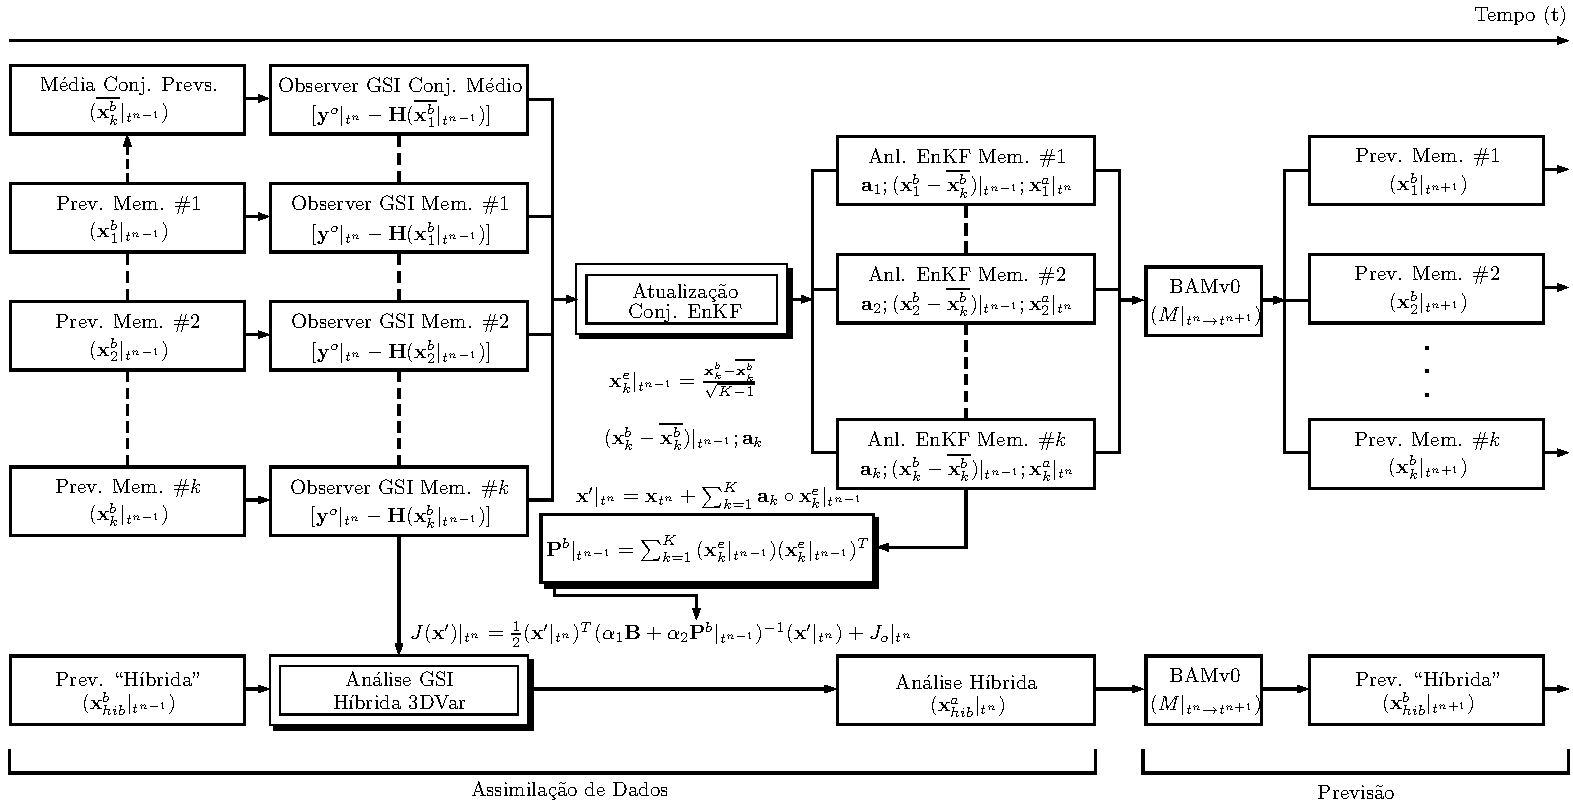
\includegraphics[width=\textwidth]{diagrama.pdf}
			\caption{Exemplo de um diagrama produzido no programa \LaTeX\textit{Draw}.}
		\end{figure}
	\end{block}
\end{frame}

\begin{tcboutputlisting}
\begin{frame}{\textit{Frames}}

    \vspace{1em}
    
    \begin{block}{Uma figura com o ambiente {\tt figure}:}
    
    \begin{figure}
        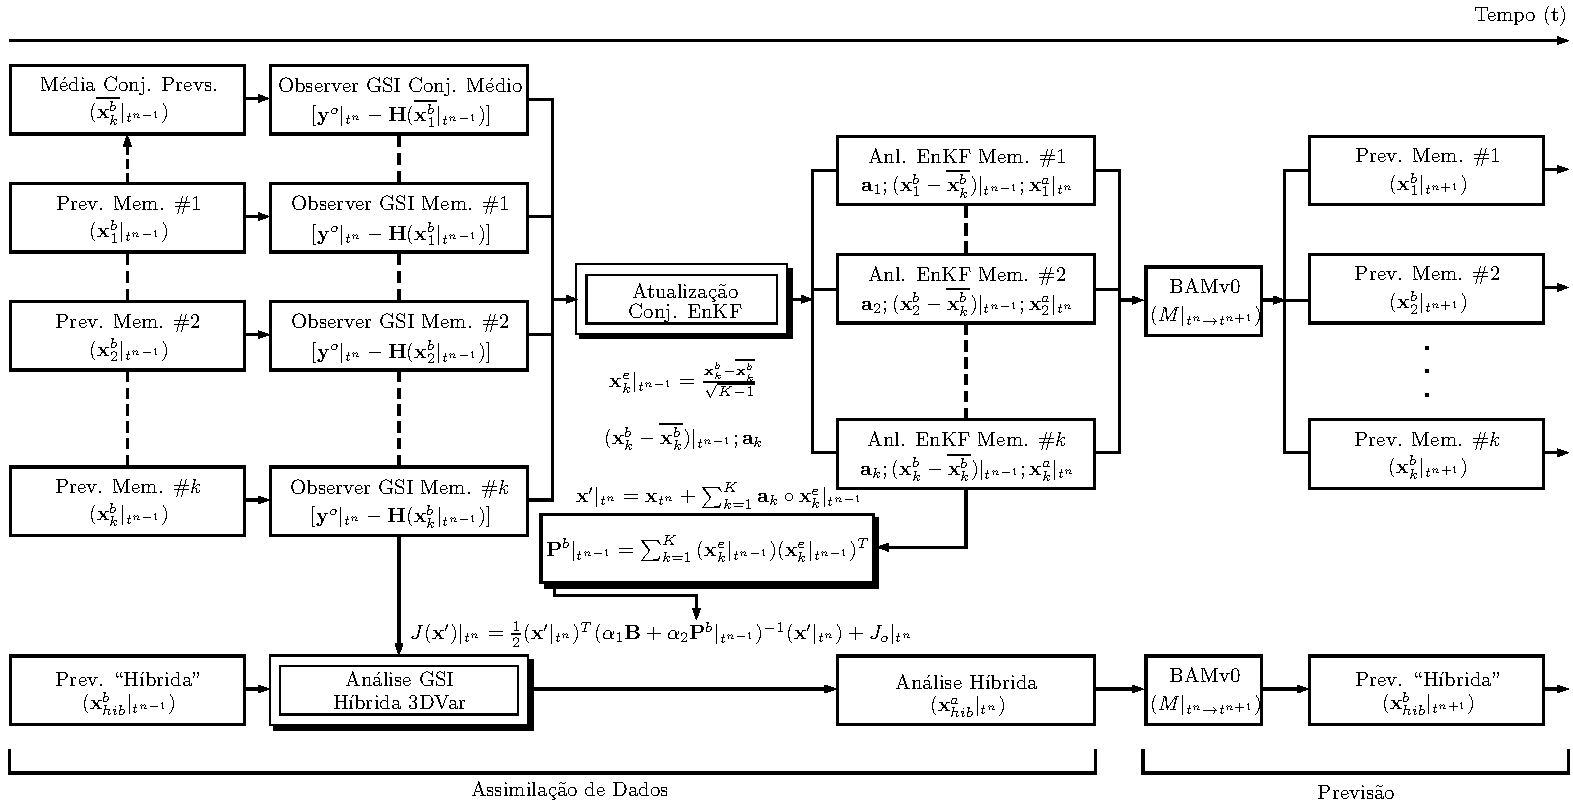
\includegraphics[scale=0.01]{diagrama.pdf}
        \caption{Exemplo de um diagrama produzido no programa \LaTeX\textit{Draw}.}
    \end{figure}
    
    \end{block}
    
\end{frame}
\end{tcboutputlisting}

\begingroup
\setbeamercolor{background canvas}{bg=InpeLaranja}
\begin{frame}[plain]{}
  \mylistingf{Código do \textit{Frame} anterior}
\end{frame}
\endgroup

\begin{frame}{\textit{Frames}}
    \begin{block}{Posicionamento dos elementos:}
        \vspace{1em}
        Assim como em um documento \LaTeX{} em que os parágrafos são justificados por padrão, os corpos flutuantes na classe do \textit{Beamer} são centralizados por padrão. Utilize a \textit{macro} {\tt vspace} para ajustar o espaçamento vertical entre os corpos flutuantes.
    \end{block}
\end{frame}

\subsection{Ambientes Especiais}

\begin{frame}{Ambientes Especiais}
    \vspace{3em}
    \begin{block}{No Beamer pode-se inserir blocos de texto com os seguintes ambientes:}
        \begin{itemize}
            \pause
            \item {\tt block}: Um bloco normal. A cor deste bloco é azul;
            \pause
            \item {\tt exampleblock}: Um bloco de exemplo. A cor deste bloco é verde;
            \pause
            \item {\tt alertblock}: Um bloco de alerta. A cor deste bloco é vermelho.
        \end{itemize}
        \pause
        \begin{marker}
            \centering
            Dependendo do tema utilizado, a configuração e a apresentação destes ambientes (blocos) pode ser sensivelmente diferente! Prefira sempre utilizar temas e esquemas de cores pré-definidos!
        \end{marker}
    \end{block}
\end{frame}

{
\setbeamercolor{background canvas}{bg=}
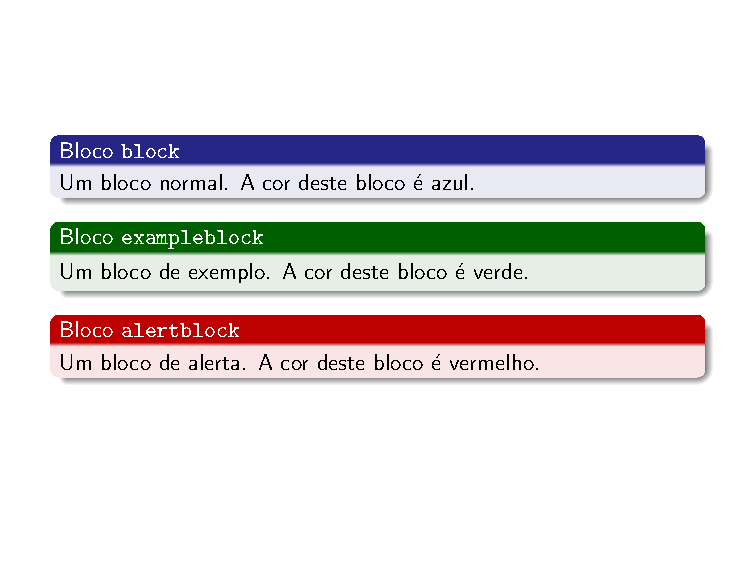
\includepdf[page=1]{./figs/blocos.pdf}
}

\subsection{Temas}

\begin{tcboutputlisting}
    \usetheme{<nome do tema>}
\end{tcboutputlisting}

\begin{frame}{Temas e Esquemas de Cores}
    \begin{block}{Selecionar um tema:}
        \begin{multicols}{4}
            \scriptsize
            \begin{enumerate}
                \item AnnArbor
                \item Antibes
                \item Bergen
                \item Berkeley
                \item Berlin
                \item Boadilla
                \item boxes
                \item CambridgeUS
                \item Copenhagen
                \item Darmstadt
                \item default
                \item Dresden
                \item Frankfurt
                \item Goettingen
                \item Hannover
                \item Ilmenau
                \item JuanLesPins
                \item Luebeck
                \item Madrid
                \item Malmoe
                \item Marburg
                \item Montpellier
                \item PaloAlto
                \item Pittsburgh
                \item Rochester
                \item Singapore
                \item Szeged
                \item Warsaw
            \end{enumerate}
        \end{multicols}
        \vspace{1em}
        \mylisting{Inlcuir no preâmbulo}
    \end{block}
\end{frame}

{
\setbeamercolor{background canvas}{bg=}
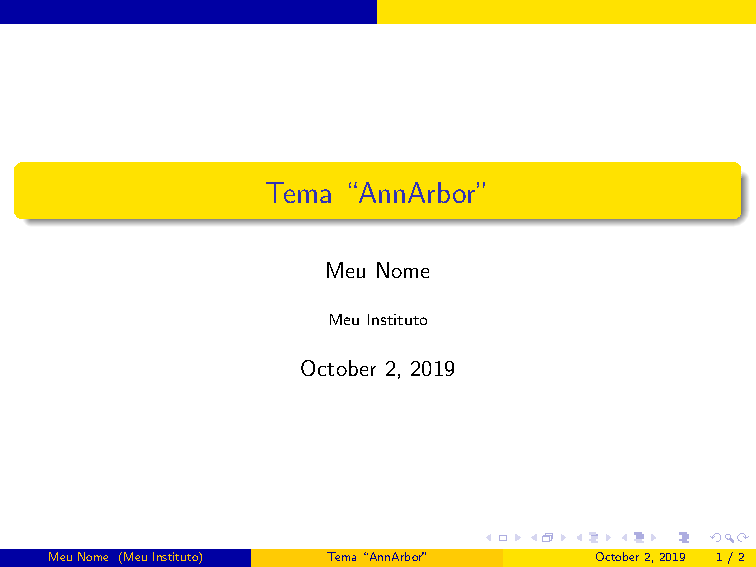
\includepdf[pages=1-56]{./figs/temas-beamer.pdf}
}

\begin{tcboutputlisting}
\beamertemplatenavigationsymbolsempty
ou
\setbeamertemplate{navigation symbols}{}
\end{tcboutputlisting}

\begin{frame}{Temas}
    \begin{block}{A barra de navegação:}
        \vspace{1em}
        Nos temas pré-definidos do \textit{Beamer}, há uma barra de navegação persistente:
        \vspace{-2em}
        \begin{figure}
            \centering
            
\includegraphics[trim={8cm 0.35cm 0 8cm}, clip,scale=1.5]{./figs/beamer-capa.pdf}
            \caption{A barra de navegação.}
        \end{figure}
    \end{block}
    %\vspace{1em}
    %\begin{alertblock}{Para removê-la, basta adicionar ao preâmbulo:}
    \mylisting{Para removê-la basta adicionar ao preâmbulo}
    %\end{alertblock}
\end{frame}

\subsection{Efeitos}

\begin{frame}{Efeitos}
    \begin{block}{Comando {\tt pause}:}
        \vspace{1em}
        O Comando {\tt pause} insere um passo entre os elementos dentro de um \textit{frame}. Por exemplo:
        \begin{enumerate}
            \pause
            \item Um item;
            \pause
            \item Outro item;
            \item Mais um item.
        \end{enumerate}
        \pause
        Percebeu? Entre os itens 1 e 2, há uma pausa; mas não há entre os itens 2 e 3!
    \end{block}
\end{frame}

\begin{tcboutputlisting}
\begin{frame}{Efeitos}
    \begin{block}{Comando {\tt pause}:}
        \vspace{1em}
        O Comando {\tt pause} insere um passo entre os elementos dentro de um \textit{frame}. Por exemplo:
        \begin{enumerate}
            \pause
            \item Um item;
            \pause
            \item Outro item;
            \item Mais um item.
        \end{enumerate}
        \pause
        Percebeu? Entre os itens 1 e 2, há uma pausa; mas não há entre os itens 2 e 3!
    \end{block}
\end{frame}
\end{tcboutputlisting}

\begingroup
\setbeamercolor{background canvas}{bg=InpeLaranja}
\begin{frame}[plain]{}
    \mylistingf{Código do \textit{frame} anterior}
\end{frame}
\endgroup

\begin{frame}{Efeitos}
    \begin{block}{Comando {\tt pause}:}
        \vspace{1em}
        O Comando {\tt pause} pode ser utilizado antes de tabelas, blocos, equações, listas, figuras etc. Mais um exemplo:
		\pause
		\begin{align}
 			x            & = 1 + 2y + 3z \\ 
			3x -  y + 2z & = 0           \\
			2x +  y      & = 2 - z             
		\end{align}
    \end{block}
\end{frame}

\begin{tcboutputlisting}
\begin{frame}{Efeitos}

    \pause

    \begin{block}{Comando {\tt pause}:}
    \vspace{1em}
        O Comando {\tt pause} pode ser utilizado antes de tabelas, blocos, equações, listas, figuras etc. Mais um exemplo:

        \pause

        \begin{align}
            x            & = 1 + 2y + 3z \\ 
            3x -  y + 2z & = 0           \\
            2x +  y      & = 2 - z             
        \end{align}
    \end{block}
\end{frame}
\end{tcboutputlisting}

\begingroup
\setbeamercolor{background canvas}{bg=InpeLaranja}
\begin{frame}[plain]{}
  \mylistingf{Código do \textit{frame} anterior}
\end{frame}
\endgroup

\begin{frame}{Efeitos}
    \begin{block}{Controlando itens:}
        \vspace{1em}
        O Comando {\tt pause} apresenta os elementos em um \textit{slide} de forma sequencial. Podemos também controlar a ordem em que os itens devem aparecer:
        \begin{enumerate}
            \item<4-> Um item;
            \item<3-> Outro item;
            \item<2-> Mais um item.
        \end{enumerate}
        \onslide<5->
        Percebeu? Entre os itens 1, 2 e 3, apareceram na ordem reversa. Esta frase apareceu apenas no útimo \textit{frame}!
    \end{block}
\end{frame}

\begin{tcboutputlisting}
\begin{frame}{Efeitos}
    \begin{block}{Controlando itens:}
        \vspace{1em}
        \pause
        O Comando {\tt pause} apresenta os elementos em um \textit{slide} de forma sequencial. Podemos também controlar a ordem em que os itens devem aparecer:
        \begin{enumerate}
            \item<4-> Um item;
            \item<3-> Outro item;
            \item<2-> Mais um item.
        \end{enumerate}
        \onslide<5->
        Percebeu? Entre os itens 1, 2 e 3, apareceram na ordem reversa. Esta frase apareceu apenas no útimo \textit{frame}!
    \end{block}
\end{frame}
\end{tcboutputlisting}

\begingroup
\setbeamercolor{background canvas}{bg=InpeLaranja}
\begin{frame}[plain]{}
  \mylistingf{Código do \textit{frame} anterior}
\end{frame}
\endgroup

\begin{frame}{Efeitos}
    \begin{block}{Comando {\tt onslide}:}
        \vspace{1em}
        \pause
        O Comando {\tt onslide} permite indicar a em qual \textit{slide} um item deverá aparecer:
        \onslide<4->
        \begin{enumerate}
            \item Um item;
            \item Outro item;
            \item Mais um item.
        \end{enumerate}
        \onslide<3-> Ué, cadê os itens que estavam aqui? \\\\
        \onslide<5-> Percebeu? A lista apareceu depois da frase acima. Repare na numeração dos \textit{frames}!
    \end{block}
\end{frame}

\begin{tcboutputlisting}
\begin{frame}{Efeitos}
    \begin{block}{Comando {\tt onslide}:}
        \vspace{1em}
        O Comando {\tt onslide} permite indicar a em qual \textit{slide} um item deverá aparecer:
        \onslide<4->
        \begin{enumerate}
            \item Um item;
            \item Outro item;
            \item Mais um item.
        \end{enumerate}
        \onslide<3-> Ué, cadê os itens que estavam aqui? \\\\
        \onslide<5-> Percebeu? A lista apareceu depois da frase acima. Repare na numeração dos \textit{frames}!
    \end{block}
\end{frame}
\end{tcboutputlisting}

\begingroup
\setbeamercolor{background canvas}{bg=InpeLaranja}
\begin{frame}[plain]{}
  \mylistingf{Código do \textit{frame} anterior}
\end{frame}
\endgroup

\subsection{Compilação}

\begin{frame}{Compilação}
\begin{block}{A compilação segue o mesmo procedimento!}
\vspace{5em}
\begin{figure}
\tikzstyle{format} = [draw, thin, fill=blue!20]
\tikzstyle{medium} = [ellipse, draw, thin, fill=green!20, minimum height=2.5em]

\resizebox{8cm}{!}{%
\begin{tikzpicture}[node distance=3cm, auto,>=latex', thick]
    % We need to set at bounding box first. Otherwise the diagram
    % will change position for each frame.
    \path[use as bounding box] (-1,0) rectangle (10,-2);
    \path[->] node[format] (tex) {Arq. {\tt .tex}};
    \path[->] node[format, right of=tex] (dvi) {Arq. {\tt .dvi}}
                  (tex) edge node {\LaTeX} (dvi);
    %\path[->, draw]<3-> (tex) -- +(0,-1) -| node[near start] {Bib\TeX} (dvi);
    \path[->, draw=blue] (tex) -- +(0,-1) -| node[near start] {\color{blue}{Bib\TeX{}}} +(2.75,-0.3) (dvi) +(-0.25,-0.3);
    
    %\path[-> draw] (tex) -- +(0,-1) -| node[near start] (dvi + (-1,-1));
    
    %\path[->, draw] (-1.5,1.5) rectangle (4.5,-2) node[above right] {$\times$2};
    \path[->] node[format, right of=dvi] (ps) {Arq. {\tt .ps}}
                  node[medium, below of=dvi] (screen) {Tela}
                  (dvi) edge node {dvips} (ps)
                        edge node[swap] {xdvi} (screen);
    \path[->] node[format, right of=ps] (pdf) {Arq. {\tt .pdf}}
                  node[medium, below of=ps] (print) {Impressão}
                  (ps) edge node {ps2pdf} (pdf)
                       edge node[swap] {gs} (screen)
                       edge (print);
    \path[->] (pdf) edge (screen)
                        edge (print);
    \path[->, draw=red] (dvi) -- +(0,2) -| node[near start] {\color{red}{dvipdf}} +(6.25,0.3) (pdf);
    \path[->, draw] (tex) -- +(0,1) -| node[near start] {pdf\LaTeX} (pdf);
\end{tikzpicture}
}
\end{figure}
\end{block}
\end{frame}

\begingroup
\setbeamercolor{background canvas}{bg=white}
\begin{frame}[plain]
  \centering
  {\Large
  OBRIGADO!
  \\ 
  \color{InpeLaranja}{\adfclosedflourishleft}
  \\ 
  \color{InpeAzul}{
  {\small \href{mailto:carlos.bastarz@inpe.br}{carlos.bastarz@inpe.br}}}
  \\
  {\small \href{https://github.com/cfbastarz}{github.com/cfbastarz}}
  }
\end{frame}
\endgroup

\end{document}
